The heuristics selected for this evaluation are formed around Lee's BNC World index~\cite{lee2003bnc}.  This selection was chosen because of their alignment to operationalisable, human-level metadata and the existence of multiple corpora with this level of annotation.



There are two main approaches to populating the corpus description using these heuristics: either read the seed corpus' contents and classify each data point, or read a list of metadata from an existing index.  The latter approach is used in this evaluation, since it is applicable to corpora with partially-missing data (such as the personal corpus data resulting from data gathering in Chapter~\ref{5}).

The accuracy of the classifiers listed here is responsible for minimising excess dispersion relative to the input corpus.  The nature of their residual error is also going to apply bias to the resulting data set.

Since many of these heuristics surround operationalising a corpus, a large body of research exists for classifying and extracting useful dimensions from texts.  The heuristics presented here are proof-of-concept only, and it is expected that the design of the heuristics used for a study is selected to match the theoretical basis of any analysis.

The heuristics presented here are document-level.  In most corpus designs, word count would be considered a measure of the size of the corpus (rather than a property of its constituents).  The method evaluated here is capable of retrieving truly IID samples at different levels, and demands a different selection of heuristics and metadata when operating at the word or sentence level.  Document level metadata are both high-level enough to be distributed for confidential corpora and descriptive enough to enable accurate retrieval (by contrast, word or part-of-speech frequencies would reveal much of the contents of the original corpus, which may not be desirable).




\subsection{Audience Level}
The BNC User's Reference Guide~\cite{CITE} describes audience level thus:

\begin{quote}
...a subjective assessment of the text's technicality or difficulty.
\end{quote}

This is expanded upon slightly by Lee~\cite{lee2003bnc}, saying:

\begin{quote}
    \textsl{Audience level}, on the other hand, is an \textbf{estimate} (by the compilers) of the \textbf{level of difficulty} of the text, or the amount of background knowledge of its subject matter which is assumed.
\end{quote}

One approach to modelling this complexity is to use word lists such as those used in education, however, this is difficult to apply to such disparate topics without extensive compilation of such lists.  A simpler approach uses metrics computed from the morphology of words to form a readability score.  Such metrics are already widely used in word processing software and for designing documents for public consumption.


The classifier used for evaluation is based on the Flesch reading ease score~\cite{flesch1948new}.  This score is widely used, easy to compute, and correlates with the simple `low/med/high' classification used in the BNC metadata:

$$
readability_{F} = 06.835 - 1.015 \left( \frac{\text{total words}}{\text{total sentences}} \right) - 84.6 \left( \frac{\text{total syllables}}{\text{total words}} \right)
$$


%Readability ranks: 
% - med: 1651 items, mean = 55.44412267430666, sd = 12.76812426643693, var = 163.02499728317557
% - low: 664 items, mean = 62.95293871760397, sd = 14.424512199650604, var = 208.06655219786907
% - high: 820 items, mean = 47.70965585209567, sd = 12.445956325065204, var = 154.90182884543054
% - ---: 914 items, mean = 82.02288020623476, sd = 20.6424573733852, var = 426.111046412025
%Classifier error: 
% - med: 1239 / 1651 = (75.04542701393095%
% - low: 226 / 664 = (34.036144578313255%
% - high: 277 / 820 = (33.78048780487805%
% - ---: 914 / 914 = (100.0%
\begin{table}[h]
    \center
    \begin{tabular}{|c|c|c|c|}
        \hline 
        $\bar{readability_{F}}$ & BNC Audience level & Standard Deviation & na\"ive acc. \\
        \hline 
        63 & Low & 14.4 & 65.9\% \\
        55 & Med & 12.7 & 25.0\% \\
        47 & High & 12.4 & 66.3\% \\
        82 & (unclassified, speech) & 20.6 & - \\
        \hline
    \end{tabular}
    \caption{Target Flesch reading ease scores and their equivalent BNC categorisation.}
    \label{tab:evaluation:heuristics:fscore}
\end{table}




%plot(density(as.numeric(as.character(dat$readability))), main="BNC World Flesch-Kincaid Readability Scores", xlab="Readability Score (bandwidth: 3.192)")

In order to establish the meaning of the BNC audience level categories in terms of this score, means were computed from the BNC world data.  These means, shown in Table~\ref{tab:evaluation:heuristics:fscore} (a reproduction of Table~\ref{tab:rebuilding:method:fscore}), were used by a simple classification algorithm that selects the category with the nearest mean value.  This na\"ive method yields the accuracy indicated in the `na\"ive acc.' column of Table~\ref{tab:evaluation:heuristics:fscore}, indicating that the readability score is not an ideal measure of the audience level.



\begin{figure}[h]
    \centering
    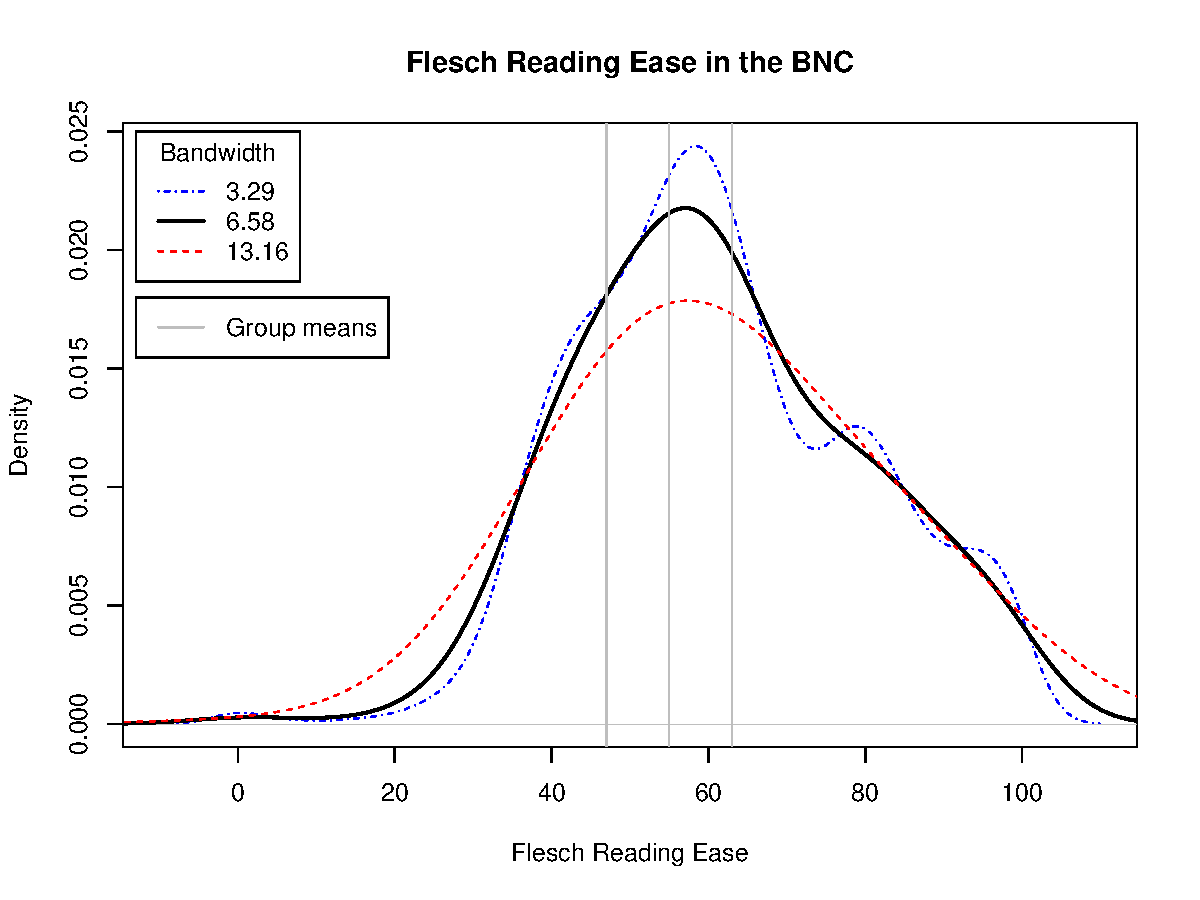
\includegraphics[width=0.8\textwidth]{evaluation/fleschbncdist}
    \caption{Flesch reading ease distribution in the BNC.}
    \label{fig:evaluation:heuristics:fleschbncdist}
\end{figure}


Rather than continue to use the categorisation used in the BNC, each text was scored for readability and the raw Flesch reading ease score used as its point within that dimension.  The `cpr' profiling tool then simply represents the underlying distribution as a continuous one (rather than artificially discretised into `high', `medium' and `low').

The standard deviation of categories within Table~\ref{tab:evaluation:heuristics:fscore} provides us with a convenient source for the bandwidth of the smoothing function used to identify the empirical distribution of the reading ease scores.  Using graphical methods (illustrated in Figure~\ref{fig:evaluation:heuristics:fleschbncdist} the value of $\sigma / 2$ was chosen to represent the distribution: this offers a tradeoff between accurately portraying the distribution and permissively selecting documents online.  This method also clarifies the difficulties associated with attempting to accurately classify audience level based on readability metrics.

Where a text is unavailable, knowledge of the standard deviation of each of the readability categories in the BNC allows us to produce an approximation of the distribution of readability scores.  This approach (as well as the smoothing above) illustrate the value of manually modifying the text distributions during the design phase.

As we are using a proxy variable to impute the reading ease, any classifier accuracy issues are deferred to the assumption that `reading ease' is something we, as corpus designers, care about.






\subsection{Word Count}
Word counts are, for our purposes, trivial to compute.  There are two challenges to operationalising word counts, however.

The former of these pertains to metadata and other boilerplate within files.  Files must be processed prior to word counts being performed.  This means (like many other tools) that we must post-process candidate files even if we elect to discard their contents.

Secondly, it is necessary to normalise deviance measures when comparison documents: this poses a particular challenge as word counts are open-ended.  The method used here was to enforce an arbitrary limit, above which any distances in the word count dimension register as $1$.  Because the sampling method does not primarily rely on gradient descent, this is fairly safe, however, selection of the threshold does impact the importance assigned to word count (vs. some other metadata dimension): too high and it will undervalue differences in word count.

The arbitrarly limit selected for the BNC was \td{limit from config file}.  This is sufficiently large that it encompasses the word counts for all BNC files, allowing for at least \td{n\%} excess.  In practice (as we shall discuss later~\td{where}) most documents fall short, and this limit could be reduced.

% --- 
It is worth noting the difference in philosophy this method embodies compared to many corpus studies: the word count here is a property of each document, and not a measure of corpus size.  Unlike many methods, we are sampling at the same level we are presuming analysis at (though this level is variable due to the ease with which documents may be selected).






\subsection{Genre}
Genre is arguably the most important single stratification applied to a general-purpose corpus (even forming the bulk of the definition of its name), yet it remains one of the more nebulous terms.  Here we follow Lee's definitions once more, commensurate with the BNC index that serves as the source of much of the metadata for our corpus definition file.

Due to the complexity of genre taxonomies (and thus the relative difficulty of classifying documents therein), there is significant motive to take the same approach as audience level above: using a self-defined or simpler taxonomy to simplify imputation or selection.  On the other hand, the BNC classification is well-known and likely to be used in any corpus augmentation task (``I want this subset of the BNC, but \textsl{more} of it.'').  We describe here an approach using the existing BNC classifications for this reason, with a detailed discussion of the implications of other options below\td{where}.


As this is a proof-of-concept system, the accuracy of the classifiers used need not be cutting-edge.  This relaxed requirement is reinforced by the notion that any errors are `sane', falling along such ambiguities as identified by Lee~\cite[p.~11]{lee2003bnc}:

\begin{quote}
It may be the case that the actual content/topic of these linguistics-relatyed texts make them seem less like social science textx than arts of applies science texts...
\end{quote}

This `sanity of error' is enforced by using a distance measure that is based on rank correlation of token type frequencies, allowing two categories to be judged on a scale more meaningful than simple boolean equality.  This luxury may not be available for all potential discrete classification systems (such as those read from external indices), and is not a requirement of convergeance to the input distribution.

The distinction between genres is often somewhat variable: some, such as \variable{w\_newsp\_brdsht\_nat\_*}, are made between the subject of texts, whereas others fall along lines of context or what others may term `text type' (\variable{W\_email} vs. \variable{W\_essay\_sch}).  This makes it particularly difficult to identify a model that linearises features within the dataset consistently enough for many classification algorithms to work well.

Lee's taxonomy is partially hierarchical, with many of the more detailed categories harbouring both this `text type' distinction as well as one regarding topic.  Both were retained here as they align to two distinct processes when sampling: the text type is an indication of (roughly) where a document may be found, and the topic regards more which document to select.





% --

\paragraph{}
The problem of identifying BNC genre from free text is a simple 70-way classification task\footnote{Such that a 70-way classification task may be described as simple at all.}.  In practice, the subjective nature of the taxonomy and the large number of classes makes this a challenging endeavour.  This is a clear illustration of the difficulties encountered using the ImputeCaT method: whilst it may not be necessary to find documents online with great accuracy, there must exist \textsl{some} method of discriminating between them in a useful way.



In his 2007 paper on web genres, Sharoff~\cite{sharoff2007classifying} fits a number of classifiers to the BNC, using a variety of genre taxonomies.  



% FIXME: edit from here.





In light of the poor accuracy of classifiers trained on the full BNC category set, this evaluation was instead performed on a sub-set of the BNC documents, aligned to the EAGLES genre categories.  Decisions such as this are impossible to comment on with regards to how they affect the value of the output corpus, except when used for a particular purpose.  Note also that it is possible to minimise the need for such compromises by careful selection of which metadata items are used to describe the corpus (though this is unlikely to be an area open to much choice).  For the purposes of evaluation, fewer categories with greater accuracy are, if anything, preferrable.

This procedure was chosen to follow that used in Sharoff's 2007 study on classifying web documents for under-resourced languages~\cite{sharoff2007classifying}.  One key difference, however, is that there is no reason to restrict ourselves to limited resource usage.

Even with a restricted parameter space, the problem of identifying genre is acknowledged as a difficult one:

\begin{quote}
The classification of texts into different genres seems to have been mostly achieved through external criteria rather than through internal, linguistic criteria.
\end{quote}\td{ cite EAGLES, \url{http://www.ilc.cnr.it/EAGLES/texttyp/node9.html}}

Interestingly, the manner of retrieval and the nature of the web offer some avenues for working with external data: It is firstly possible to retrieve documents according to an existing genre directory, all but guaranteeing a fit.  Further, HTML and HTTP metadata and stylistic properties of web documents (or those which are closely linked) may indicate genre as (or more) effectively as linguistic content.  These are all places where further research dovetails with the methods described here to increase overall accuracy.



\paragraph{Na\"ive Bayes}
This classifier basically doesn't work.


\paragraph{Unigram Frequency Rank Correlation}
This classifier works if you do certain things.  Spearman correlation based (Mann-Whitney).

\paragraph{Ngram Frequency Rank Correlation}
This classifier is particularly slow due to the large library of ngrams that are stored for each class, and the overhead required to read these from backing store.  In practice this makes document classification often slower than download.


\paragraph{}





* Classifier description
* Talk about rationality of errors
* Talk about how difficult this is
* Evaluate unigram, ngram, naive bayes
* Comment on the choice of genres, how artificial or simple ones might be better (perhaps aligned with data source such as DMOZ?)



